\documentclass[a4paper, titlepage]{book}
\usepackage{frontespizio}
\usepackage{graphicx}       % per inserire le immagini
\graphicspath{{../pdf/}{C:\Users\aldob\Documents\tesi\images}}

\usepackage{cite}          % per poter citare
\usepackage[italian]{babel} %lingua
\usepackage{url}
%\usepackage[lighttt]{lmodern}
%\usepackage{listings}% per inserire codice python

\usepackage{listings}
\usepackage{xcolor}

\definecolor{codegreen}{rgb}{0,0.6,0}
\definecolor{codegray}{rgb}{0.5,0.5,0.5}
\definecolor{codepurple}{rgb}{0.58,0,0.82}
\definecolor{backcolour}{rgb}{0.95,0.95,0.92}
\lstdefinestyle{mystyle}{
    backgroundcolor=\color{backcolour},   
    commentstyle=\color{codegreen},
    keywordstyle=\color{magenta},
    numberstyle=\tiny\color{codegray},
    stringstyle=\color{codepurple},
    basicstyle=\ttfamily\footnotesize,
    breakatwhitespace=false,         
    breaklines=true,                 
    captionpos=b,                    
    keepspaces=true,                 
    numbers=left,                    
    numbersep=5pt,                  
    showspaces=false,                
    showstringspaces=false,
    showtabs=false,                  
    tabsize=2
}

\lstset{style=mystyle}


\usepackage{fancyhdr}   %linee nell'head dopo la prima pagina di ogni capitolo
\pagestyle{fancy}
\addtolength{\headwidth}{\marginparsep}
\renewcommand{\chaptermark}[1]{\markboth{#1}{}}
\renewcommand{\sectionmark}[1]{\markright{\thesection\ #1}}
\fancyhead[LE,RO]{\bfseries\thepage}



\usepackage{hyperref}     %per poter cliccare i link
%\hypersetup{colorlinks=true, citecolor=blue}   % colore capitoli dell'indice

\begin{document}


\begin{frontespizio}

\Universita{Torino}
\Logo[3.5cm]{images/logo universita.png}
\Dipartimento{INFORMATICA}
\Corso[Laurea]{Informatica}
\Titoletto{Tesi di laurea}
\Titolo{IoT su piattaforma Raspbian/Raspberry:\\
Sviluppo di una cassetta delle lettere smart
}
\Relatore{Prof.~Michele Garetto}
\Candidato[847091]{Aldo~Bushaj}
\Annoaccademico{2019-2020}

\end{frontespizio}


\tableofcontents

\frontmatter
\chapter{Abstract}
\label{ch:abstract}
Oggigiorno tra ufficio, hobby e impegni vari trascorriamo sempre meno tempo a casa, quindi a volte, se si aspetta una lettera importante o semplicemente per
comodità, l'deale sarebbe che qualcuno o meglio qualcosa avvisi l'utente (il proprietario della cassetta delle lettere) ogni qualvolta viene ricevuta nuova 
posta informandolo eventualmene anche dell'identità del mittente.

Usando il prototipo sviluppato, quando il mittente inserisce una lettera nel bucalettere, una fotocamera scatta una foto che verrà caricata nel database. A questo
punto, tramite un'email all'indirizzo precedentemente impostato, l'utente viene notificato dell'avvenuta ricezione di nuova posta indicandone anche l'identità.

Il progetto è stato implementato su una scheda Raspberry-Pi, mentre l'applicazione, è stata scritta usando il linguaggio Python.
Sono stati utilizzati diversi servizi di AWS (Amazon Web Services) sia per quanto riguarda il riconoscimento facciale che per il caricamento delle foto scattate nel 
database, i più importanti sono:
\begin{itemize}
    \item Amazon Rekognition
    \item Amazon Simple Storage Service (Amazon S3)
    \item Amazon DynamoDB
    \item AWS Lambda 
\end{itemize} 
\chapter*{Ringraziamenti}
\label{ch:ringraziamenti}


\null\vspace{\stretch{1}}

%\ChTitleVar{\LARGE\bfseries\rm\centering}
\begin{flushright}
    \Large\textit{\itshape{Un ringarziamento va ai miei genitori, ai miei fratelli e a tutti gli amici e familiari che mi hanno sostenuto in questo periodo.}}
\end{flushright}

\vspace{\stretch{2}}\null


\mainmatter
\chapter{Introduzione}
\label{ch:introduzione}
Internet, è una piattaforma globale che permette a oggetti di tutti i giorni di coordinarsi e comunicare tra loro. È in quest'ottica che nasce 
Internet of Things, (IoT, Internet delle cose in italiano), la quale indica un trend attuale che prevede la connessione a Internet di ogni tipologia di oggetto fisico, 
anche alcune finora impensabili.

Oggigiorno è possibile collegare qualsiasi cosa, dagli oggetti familiari, come frigoriferi e lampadine, a risorse aziendali quali 
le etichette di spedizioni e i dispositivi medici, fino ai dispositivi indossabili, ai dispositivi intelligenti e alle città smart, la cui esistenza è esclusivamente 
dovuta all'IoT.

I primi concetti alla base dell’IoT sono stati abbozzati nel 1982, quando alcuni ricercatori della Carnegie Mellon University hanno applicato sensori
e la connessione in rete a un distributore di bibite dell’Ateneo per conoscernene lo stato di funzionamento. 

Il termine ``Internet of Things" fu coniato, però, per la prima volta solo nel 1999 dall'imprenditore inglese Kevin Ashton per descrivere la connessione di oggetti del 
mondo fisico ad Internet, Kevin mostra i limiti di una tecnologia basata solo sulle idee, su dati generati dagli utenti e vede, invece, le prospettive che possono 
offrire gli oggetti di tutti i giorni connessi in rete, in grado di fornirci informazioni sul loro stato, permettendoci quindi di sapere quando uno di essi necessita 
di essere riparato o sostituito.

A oggi, come si può notare dal grafico in Figura~\ref{IOTgraph}, il numero di dispositivi connessi è in continua crescita, anche perchè i campi di applicazione sono numerosi, 
questo grazie alle enormi potenzialità che oggetti di tutti i giorni possano offrirci se connessi a Internet e/o interconnessi tra di loro equipaggiandoli 
all'occorenza con svariati sensori.
I campi in cui Internet of Things si è affermato maggiormente sono i seguenti:
\begin{itemize}
    \item Domotica
    \item Smart City
    \item Industria
    \item Agricoltura
    \item Logistica e trasporto
\end{itemize}
\begin{figure}[htb]
    \centering
    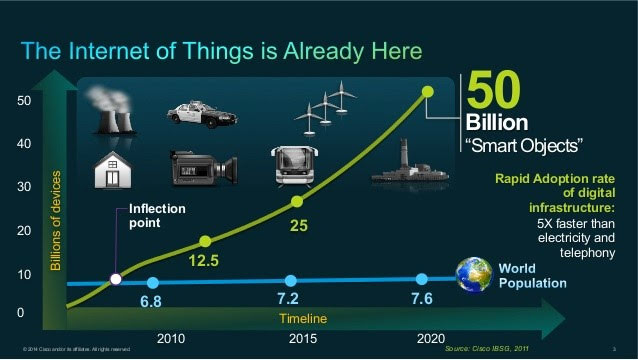
\includegraphics[width=0.7\textwidth]{images/IoT-graph.png}
    \caption{Grafico crescita del numero di dispositivi connessi.}
    \label{IOTgraph}
\end{figure}
Un report di Business Insider Intelligence~\cite{insiderIntelligence} afferma che, nei prossimi cinque anni arriveremo a 40 miliardi di dispositivi IoT mentre
i governi , entro il 2023, investiranno circa 900 miliardi di dollari per lo sviluppo di smart city, smart utility e sistemi di telecamere connesse. 
Negli Usa i dispositivi domestici smart supereranno il miliardo entro il 2023, con un consumo stimato di circa 725 dollari per famiglia, per un totale di oltre 
90 miliardi di dollari in spese per soluzioni IoT. Numeri in crescita anche nel settore industriale, infatti le imprese continueranno a investire miliardi nel settore , 
in particolare , entro il 2023 la spesa annuale per la produzione di soluzioni IoT raggiungerà circa 450 miliardi di dollari, mentre la base installata totale di sistemi 
robotici industriali raggiungerà i 6 milioni in tutto il mondo.

Stando ai dati sopra riportati ci sarà un forte aumento dei dispositivi connessi e conseguentemente aumenteranno anche i dati prodotti. Purtroppo, a fronte di uno 
scenario che fa crescere le opportunità di business e di ricchezza aumenteranno anche le minacce che porteranno ad un problema sia per quanto riguarda la sicurezza 
in generale che per quella associata alla protezione dei dati personali.

La società di ricerca Gartner nello studio “Worldwide IoT security spending forecast 2018-2021 per segment” porta l’attenzione sui rischi e sulle vulnerabilità 
collegate alla diffusione dell’Internet delle cose, pericolo alimentato peraltro anche dalla semplicità delle componenti informatiche integrate in elettrodomestici (se
si parla delle smart Home) e altri oggetti abilitati dall’IoT, unitamente a difetti della gestione e dell’aggiornamento, infatti come riportato 
nell'articolo~\cite{articoloSicurezza} negli ultimi tre anni un’azienda su 5 ha subito almeno un attacco ai propri ambienti Internet of Things. 

Il rischio per la sicurezza non riguarderà più solo server, computer o device mobili in dotazione al personale, ma tutti gli oggetti intelligenti 
che raccolgono dati e aiutano a governare edifici, produzioni, e apparti dai quali dipendono servizi di mobilità, rischio divenuto realtà quando ad esempio 
una variante del malware Mirai, chiamata OMG ha colpito gli endpoint IoT consentendo a malintenzionati di portare avanti attacchi Denial of Service su 
larga scala (dove i dispositivi infettati generavano traffico fittizio per saturare siti e servizi).

Nei prossimi anni le piattaforme IoT rischiano quindi di essere sempre più frequentemente soggette ad attacchi informatici via via più sofisticati. 
Le modalità di difesa possono essere: 
\begin{itemize}
    \item Scegliere prodotti IoT affidabili dotati di protezioni specifiche.
    \item Curare le configurazioni dei dispositivi usando credenziali di autenticazione (password) più sicure
    e assicurando l’applicazione delle patch, aggiornando sistemi operativi, driver e programmi di gestione.
    \item Cifrare i dati trasmessi da un punto all'altro implementando uno dei tanti protocolli crittografici.
    \item Analizzare i possibili attacchi in quanto , a volte , vengono attuati attacchi pensati specificamente per compromettere determinate aziende o determinate 
    attività. E’ quindi necessario progettare e applicare forme di protezione personalizzate e specificatamente indirizzate a proteggere aziende anche da precise minacce.
    \item A livello di rete si può invece limitare al minimo indispensabile la banda e altri servizi accessibili ai dispositivi IoT, quindi rilevare e segnalare 
    agli amministratori le anomalie riconducibili a possibili infezioni.
\end{itemize}
\chapter{Progetto}
\label{ch:job_motivation}
Il progetto sviluppato durante il tirocinio presso l'Universtià degli studi di Torino, con la supervisione del professore Michele Garetto, si pone come obiettivo 
quello di creare una cassetta delle lettere smart, la quale ogni volta in cui viene ricevuta posta è in grado di avvertire e far interagire l'utente 
grazie all'invio di e-mail a un specifico indirizzo preimpostato.

Per fare ciò, sono stati utilizzati diversi servizi illustrati nel dettaglio nel seguente paragrafo.


\section{Soluzione Proposta}
\label{sec:solution}
La soluzione proposta in questa tesi utilizza una ``classica" cassetta delle lettere resa smart grazie all'integrazione di diversi sensori e servizi alla scheda 
Raspberry Pi 3 Model B, di seguito verrà illustrato il suo funzionamento.

Il soggetto che invia la posta dovrà semplicemente inserire la lettera nel bucalettere, a questo punto vengono innescati una serie di eventi:
\begin{itemize}
    \item Grazie al sensore di prossimità Qwiic Proximity Sensor (VCNL4040), in Figura~\ref{photo_sensor}, viene rilevato il passaggio di un'oggetto, la lettera nel 
    nostro caso, quindi viene scattata una foto con la Raspberry Pi Camera~\ref{photo_camera}.
    \item Quindi vi è l'interazione con alcuni servizi di AWS(Amazon Web Services), in particolare, la foto appena scattata viene caricata in Amazon S3, questo evento
    lancia la funzione Lambda la quale verifica se le foto caricata è un volto riconosciuto da Amazon Rekognition e quindi presente in Amazon Dynamodb.
    \item A questo punto possono verificarsi solo due casi:
    \begin{itemize}
        \item Il volto è stato riconosciuto, quindi viene inviata una e-mail che notifica la ricezione di nuova posta con il nome del mittente.
        \item Il volto non è stato riconosciuto, quindi viene inviata un'e-mail che notifica la ricezione di nuova posta con allegata
        la foto del mittente.
    \end{itemize}
    \item Infine l'utente potrà insierire i volti non riconosciuti da Amazon Rekognition nei database inoltrando l'email ricevuta, inserendo nel corpo dell'e-mail 
    la parola chiave ADD seguita da nome e cognome con cui si vuole memorizzare il volto. Quindi dopo gli opportuni controlli, i volti inseriti saranno pronti 
    ad un prossimo eventuale controllo ad essere riconosciuti.
\end{itemize} 

Tutto il codice e funzionamento nel dettaglio del progetto verrano illustrati nel capitolo ~\ref{ch:development}.
\chapter{Tecnologie utilizzate}
\label{ch:technologies}
Per lo sviluppo del progetto sono stati implementati diversi componenti sia lato hardware che software. 
In questo capitolo verranno riportate tutte le tecnologie adottate illustrandone una breve dscrizione.

\section{Raspberry}
\label{sec:raspberry}
Per la realizzazione della ``\texttt{cassetta delle lettere smart}'' (esposta nella Sezione ~\ref{sec:solution}) inizialmente si era pensato di utilizzare la piattaforma 
hardware Arduino \footnote{https://store.arduino.cc/arduino-uno-rev3}, successivamente si è optato però per la scheda Raspberry Pi in quanto quest'ultima più 
performante e meglio equipaggiata rispetto Arduino.

In particolare è stata utilizzata una scheda RaspberryPi 3 Model B \footnote{https://www.raspberrypi.org/products/raspberry-pi-3-model-b/} illustrata in 
Figura~\ref{photo_raspberry}.

Sviluppato dalla fondazione britannica no-profit Raspberry Pi Foundation il 29 Febbraio del 2012~\cite{stroyOFraspberry_Raspbian}, il progetto nacque per stimolare 
l'insegnamento dell'informatica e della programmazione nelle scuole e per promuovere lo studio del linguaggio di programmazione Python, da cui ne deriva la sigla 
Pi del logo.
Questa scheda fra l'altro ebbe successo anche grazie al bassissimo costo, infatti le prime due versioni costavano solo 25 e 35 dollari, rispettivamente 
per la versione da 256 e 512 Mb di RAM.
\begin{figure}[htb]
    \centering
    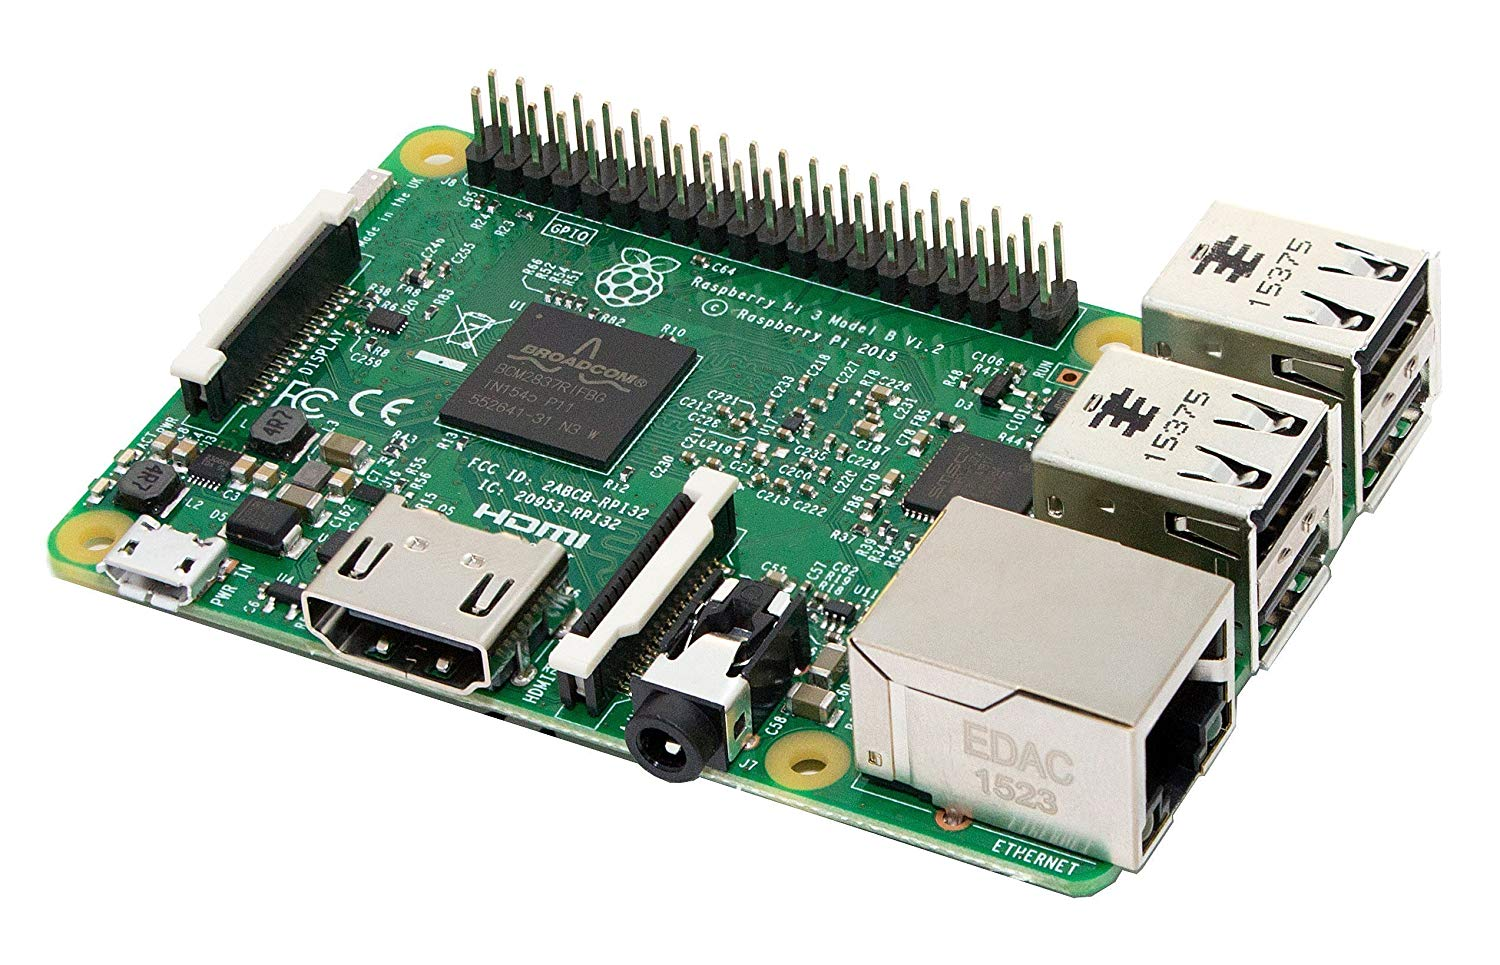
\includegraphics[width=0.7\textwidth]{images/raspberryPI.png}
    \caption{Raspberry Pi 3 Model B.}
    \label{photo_raspberry}
\end{figure}

Le specifiche tecniche della scheda Raspberry Pi 3 Model B sono:
\begin{itemize}
    \item Tensione di alimentazione: \textit{5V/2.5A DC}
    \item SoC: \textit{Broadcom BCM2837 Quad Core Cortex-A53 a 1.2 GHz, 32 kB L1 e 512 kB L2}
    \item GPU: \textit{Broadcom VideoCore IV Dual Core a 400 MHz}
    \item RAM: \textit{1GB LPDDR2 a 900 MHz}
    \item Rete: \textit{Ethernet 10/100, WiFi b/g/n 2.4 GHz, Bluetooth 4.1 con Bluetooth Low Energy(per un consumo di energia ridotto)}
    \item Porte: \textit{microSD, HDMI 1.4 CEC, jack 3.5 mm, 4 porte USB 2.0 (SMSC LAN9514)}
    \item Interfacce: \textit{CSI Camera Connector, DSI  Display Connector, GPIO header 40-pin}
    \item \textit{Slot per memoria microSD su cui viene installato il sistema operativo}
    \item Dimensioni: \textit{85 x 56 x 17 mm}
\end{itemize}

Le linee GPIO (General Purpose Input/Output), in FIgura~\ref{photo_gpio}
\footnote{www.element14.com/community/docs/DOC-73950/l/raspberry-pi-3-model-b-gpio-40-pin-block-pinout}, 
sono dei collegamenti tra il processore e i pin del 
connettore della scheda. Queste linee possono essere programmate per funzionare sia come porte di ingresso che come porte di uscita.

\begin{figure}[htb!]
    \centering
    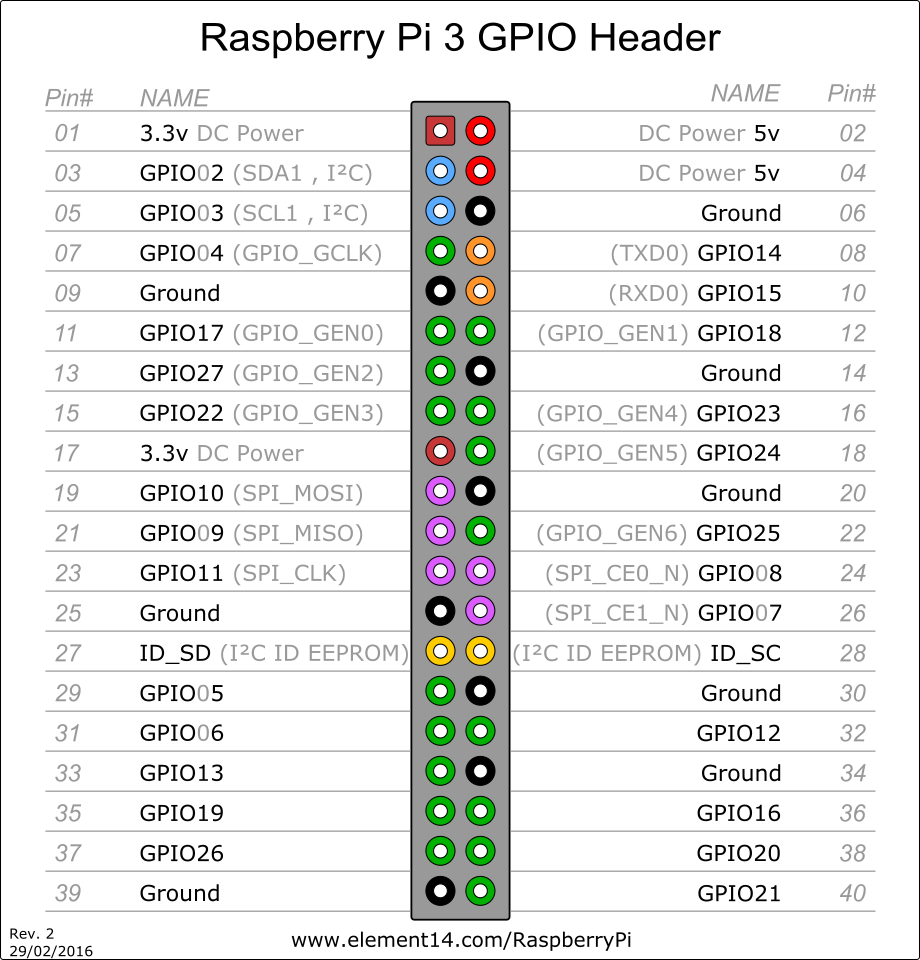
\includegraphics[width=0.7\textwidth]{images/gpio.png}
    \caption{Pin GPIO (General Purpose Input Output).}
    \label{photo_gpio}
\end{figure}

I 40 GPIO offerti dalla scheda Raspberry includono pin digitali, SPI, I2C e alimentazione 3V e 5V, esistono due differenti modalità per indicare uno specifico pin , il 
sistema BOARD ed il sistema BCM.

Il sistema BOARD fa riferimento alla loro posizione fisica, quindi effettivamente, il pin 1 risulterà essere 3.3V PWR, mentre ad esempio, riferendoci al pin 16 interagiremo 
con il pin GPIO23 (GPIO\textunderscore GEN4).

Il sistema BCM, invece,  si riferisce ai pin GPIO che sono stati direttamente collegati al SoC(``cervello'' del Pi) della scheda ed avrà quindi un modo 
differente per chiamare lo stesso pin. Ad esempio, il pin in posizione 16 visto prima, sarà chiamato GPIO23.

Per usare questi pin con questi protocolli, sono state importate una delle tante librerie Python disponibili, infine, sono state abilitate le interfacce usando l’applicazione 
Raspberry Pi Configuration disponibile nel sistema operativo Raspbian, nel menu Preferenze.


\subsection{Rasbian}
Per la scheda Raspberry è stato installato il sisitema operativo ufficiale Rasbian, identificato dall'immagine in Figura~\ref{photo_raspbian}, una 
distribuzione di Linux Debian costruita appositamente per il Raspberry Pi, il nome nasce dalla contrazione dei termini Raspberry Pi e Debian, sviluppato da 
Mike Thompson e Peter Green nel Giungno del 2012~\cite{stroyOFraspberry_Raspbian} con una build iniziale di oltre 35.000 pacchetti precompilati di software in bundle
in un formato adatto per una semplice installazione sulla scheda.

Rispetto Debian, Raspbian alleggerisce notevolmente il carico della CPU nell'esecuzione del sistema grazie a importanti modifiche dell'interfaccia grafica, questo 
anche date le limitate prestazioni della scheda. 
\begin{figure}[htb]
    \centering
    
\includegraphics[width=0.7\textwidth]{images/raspbian.png}
    \caption{Logo Raspbian.}
    \label{photo_raspbian}
\end{figure}

Per quanto riguarda le funzionalità offerte, questo è un sistema operativo discretamente completo, infatti grazie a un costante sviluppo la quantità dei software 
presenti è continuata a crescere arrivando a contenere persino programmi di elaborazione di testi o client di posta elettronica.


\subsection{Raspberry Pi Camera}
La fotocamera utilizzata per scattare le foto del mittente è la Raspberry Pi camera Module V2, in Figura~\ref{photo_camera}, un prodotto ufficiale della Raspberry Pi 
Foundation, il modello originale da 5 megapixel è stato rilasciato nel 2013 mentre quello utilizzato nel progetto è stato rilasciato nell'Aprile del 2016.

Dotata di un sensore di alta qualità da 8 megapixel Sony IMX219 appositamente disegnato con obiettivo a fuoco fisso è in grado di scattare foto da 3280x2464 pixel e 
supporta video da 1080p30, 720p60 e 640x480p60/90, si installa sulla scheda Raspberry tramite l'interfaccia CSi appositamente dedicata tramite il cavo flessibile in 
dotazione, è molto comoda e poco ingombrante grazie al ridotto peso di 3g con una grandezza pari a 25mm x 23mm x 9mm.
\begin{figure}[htb]
    \centering
    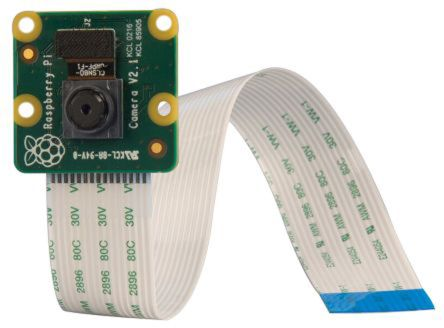
\includegraphics[width=0.7\textwidth]{images/piCamera.png}
    \caption{Raspberry Pi camera Module V2.}
    \label{photo_camera}
\end{figure}


\subsection{Qwiic Proximity Sensor (VCNL4040)}

Come illustrato nella sezione~\ref{sec:solution}, l'utente viene avvisato della ricezione di nuova posta ogni volta in cui viene introdotta una lettera nel bucalettere,
per rilevarne il passaggio è stato utilizzato il sensore Qwiic Proximity Sensor (VCNL4040), in Figura~\ref{photo_sensor}, un semplice sensore a infrarossi in grado di 
rilevare il passaggio di oggetti fino ad una distanza di circa 20cm.
\begin{figure}[htb]
    \centering
    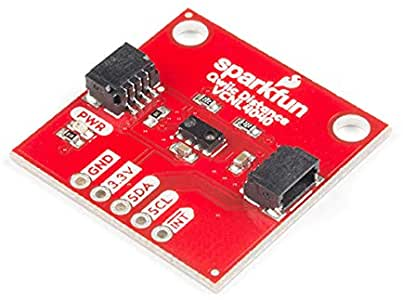
\includegraphics[width=0.7\textwidth]{images/sensor.png}
    \caption{Sensore di prossimità a infrarossi Qwiic VCNL4040.}
    \label{photo_sensor}
\end{figure}

Il sensore non ha punti morti, è in grado quindi di rilevare il passaggio di oggetti vicinissimi non determinandone una distanza esatta ma indicando se l'oggetto è più 
vicino o lontano rispetto l'ultima lettura effettuata, problema che non sussiste dal momento che sarà sufficente rilevare solo il passaggio 
della lettere senza specificare a quale distanza sia passata.



\section{Python}
\label{sec:python}
Il linguaggio di programmazione utilizzato per la realizzazione di questo progetto è Python, in particolare la versione 3.6.

Nel 1991 Guido Van Rossum, avute alcune idee mirate al miglioramento di ABC~\footnote{https://it.wikipedia.org/wiki/ABC\_(linguaggio)}, si mise a lavorare allo 
sviluppo di un nuovo linguaggio di programmazione, nasce così Python, la scelta del nome venne influenzata dalla passione dello sviluppatore per il gruppo comico 
inglese Monty Python.

Python è un linguaggio multi-paradigma che riesce a sfruttare il paradigma object oriented, la programmazione strutturata così come la  programmazione funzionale, le 
variabili sono non tipizzate e viene usata l'indentazione per definire il corpo di metodi, cicli, classi ecc\dots

Il controllo dei tipi viene eseguito a runtime ed è di tipo forte (strong typing~\footnote{https://it.wikipedia.org/wiki/Tipizzazione\_forte}), le variabili in questo 
linguaggio sono paragonabili a dei contenitori ai quali viene associato un nome, il quale consente di riferirsi in ogni momento alla variabile(contenitore) associata, 
ogni contenitore è associabile a diversi altri contenitori anche di altro tipo(String, Int, Double, ecc\dots) durante il suo tempo di vita, cioè fino a quando il 
garbage collector procede alla liberazione automatica della memoria non appena si verificano le opportune condizioni.

Python è oggi uno dei linguaggi più utilizzati in assoluto per l'estrema capacità di adattamento a tutte le esigenze e quindi applicabile in svariati ambiti, ad
esempio lo si può utilizzare per la programmazione di interfaccie grafiche(GUI) o sviluppo Web.
Nel corso del tempo si è assistito ad una vera e propria evoluzione del linguaggio, questo soprattutto dovuto al fatto d'essere open source e quindi tutti hanno 
contribuito a migliorarlo, la sua diffusione è dovuta anche a diversi vantaggi offerti, tra i tanti infatti Pyton:
\begin{itemize}
    \item È facile da usare in quanto la sintassi e i diversi moduli e funzioni che sono già inclusi nel linguaggio sono consistenti, intuitivi, e facili da imparare.
    \item È ricco di librerie con una collezione di oltre 200 moduli per svolgere i compiti più disparati.
    \item È performante, i programmi infatti vengono automaticamente compilati in un formato chiamato bytecode (formato più compatto ed efficiente, 
    garantisce quindi prestazione elevate) prima di essere eseguiti.
    \item È portabile, viene utilizzato su svariate piattaforme come : Windows, Linux, Unix, Macintosh e su cellulari Android e iOS, lo stesso codice quindi può essere 
    eseguito su qualsiasi piattaforma purché abbia l'interprete Python installato.
\end{itemize}



\section{Librerie utilizzate}
\label{sec:library}
Come fatto presente nella sezione~\ref{sec:python} è stato utilizzato Python come linguaggio di programmazione, sono state utilizzate varie librerie riportate in 
dettaglio nelle sezioni a seguire per vari scopi fra cui:
\begin{itemize}
    \item Interagire con il sensore e la fotocamera collegati alla scheda Raspberry Pi 3 Model B.
    \item Avere accesso ai servizi offerti da AWS.
    \item Utilizzare i server e-mail per inviare e ricevere e-mail.
    \item Far scattare un contatore che tiene conto del tempo trascorso e quindi eseguire delle operazioni preimpostate.
\end{itemize}


\subsection{Boto3}
\label{sec:boto3}
Boto è il Software Development Kit (SDK) di Amazon Web Services (AWS) per Python, che consente agli sviluppatori Python di scrivere software che utilizza servizi 
come Amazon S3 e Amazon EC2, per utilizzarlo come consultabile nell'appostia guida~\cite{boto3}, è stato insatallato in locale(sulla scheda Raspberry) con il comando
\textbf{pip install boto3 } e succesivamente configurato opportunamente.

Boto3 è un'applicazione che fornisce supporto nativo in Python, offre un'API orientata agli oggetti facile da usare e un accesso diretto al 
servizio di basso livello, vengono messi a disposizione due livelli di API: 
\begin{enumerate}
    \item Le API client (o di "basso livello") che forniscono mappature univoche alle operazioni API HTTP.
    \item Le API di risorse (o di "alto livello") che eseguono chiamate di rete esplicite, fornendo oggetti e raccolte di risorse per accedere agli attributi 
    ed eseguire azioni.
\end{enumerate}
Numerose richieste che utilizzano boto3 non sono istantanee, in alcuni casi questo non è un prblema, infatti è possibile fare una richiesta e controllare in un secondo
momento se è stata completata o meno, in altri casi invece, desideriamo attendere il completamento della richiesta prima di passare alle parti successive dello 
script che potrebbe fare affidamento ad un processo più lungo per essere completato, in questi casi è possiblie utilizzare dei ``waiter'' inclusi in Boto3, 
i quali ricercano in modo continuo eventuali modifiche agli stati predefiniti nelle risorse AWS, un esempio potrebbe essere quello di uno script che copia un AMI
(Amazon Machine Image)~\footnote{https://docs.aws.amazon.com/it\_it/AWSEC2/latest/UserGuide/AMIs.html}
su un altro account condividendo tutte le istantanee. Dopo aver condiviso le istantanee con l'altro account, è necessario attendere il completamento delle copie 
dell'istantanea locale prima di registrare l'AMI nell'account di ricezione.


\subsection{E-mail}

E-mail è una libreria che permette la gestione di messaggi di posta elettronica, inclusi MIME e gli altri documenti basati sulla RFC 2822, divide l'analisi e la 
generazione del messaggio di e-mail dal modello oggetto di rappresentazione interno dell'e-mail. 
Il package e-mail non è specificamente progettato per nessun invio di messaggi di posta tramite server SMTP (RFC 2821), questa è la funzione del modulo smtplib 
utilizzato in questo progetto come vedremo più avanti.

Il componente centrale del pacchetto è un "modello a oggetti" che rappresenta i messaggi di posta elettronica, un'applicazione interagisce con il pacchetto 
principalmente attraverso l'interfaccia del modello a oggetti definita nel sottomodulo dei messaggi eseguendo diverse operazioni come ad esempio rimuovere gli 
oggetti secondari dai messaggi, riorganizzare completamente il contenuto, etc\dots

Ci sono altri due componenti fondamentali del package e-mail e sono, l'analizzatore (il parser) e il generatore.
Il parser accetta in input la versione serializzata di un messaggio di posta elettronica (uno stream di bytes) e li converte in un albero di oggetti EmailMessage,
il generatore prende un EmailMessage e lo trasforma in un flusso di byte serializzato, sono presenti anche utili sotto classi per alcuni tipi di oggetti MIME comuni, 
ed alcune utilità generiche che aiutano con alcuni compiti comuni.

In questo progetto, è stato necessario avere la possibilità di inviare e 
ricevere posta elettronica, per far ciò sono state usate due librerie, smtlib\footnote{https://docs.python.org/3/library/smtplib.html} per l'invio di posta elettronica
mentre imaplib\footnote{https://docs.python.org/2/library/imaplib.html} per la ricezione.

\subsection{Picamera}
Questo pacchetto fornisce un'interfaccia Python per la videocamera Raspberry Pi, è disponibile in diverse verisoni, Python 2.7 (o versioni successive) 
o Python 3.2 (o versioni successive), il codice è concesso in licenza da BSD license~\footnote{https://opensource.org/licenses/BSD-3-Clause}.

Utilizzando questa libreria è possibile scrivere dei programmi che ci permettono di scattare immagini, girare filmati per poi elaborarli successivamente, 
inoltre grazie ai pin GPIO è possibile integrare l’uso della telecamera con sensori o interruttori.

\subsection{Adafruit vcnl4040}

Questa è la libreria di sensori di prossimità e luce ambientale Adafruit VCNL4040, sviluppata da Kattni Rembor, è stata testata e funziona perfettamente con 
il sensore adottato.

Il chip scelto ha bisogno di 2 pin per interfacciare Adafruit e utilizza il protocollo I2C per comunicare, creato da Philips, 
questo protocollo di comunicazione seriale sincrono, permette a diversi dispositivi lo scambio di dati utilizzando solo due fili collegati negli appositi pin GPIO,
in FIgura~\ref{photo_gpio}, uno viene utilizzato per l'invio dei dati mentre l'altro per sincronizzare la comunicazione.
 
\subsection{Time}

La libreria Time offre varie funzioni della libreria in linguaggio C per la maipolazione di date e tempo, visto che è legato all'implementazione in C, 
alcuni dettagli (come l'inizio dell'epoca ed il valore massimo di data supportato) sono specifiche alla piattaforma.

L'istante da cui inizia il conteggio del tempo e dato da ``epoch'', le funzioni in questo modulo non gestiscono i tempi e le date prima di ``epoch'' o molto lontane 
nel futuro, per i sistemi Unix epoch è il 1970, per cui ad esempio il primo gennaio di quell'anno, all'ora 0, il tempo trascorso da epoch è 0, mentre il punto di 
interruzione nel futuro, sempre nei sistemi Unix, è di solito l'anno 2038.


\section{Amazon Web Services}
\label{sec:aws}
Amazon Web Services (o AWS), azienda statunitense di proprietà del gruppo Amazon, è una piattaforma che offre servizi in cloud computing, rivolta a tutte quelle
imprese o Pubbliche Amministrazioni che intendono innovare e potenziare il loro reparto IT e la loro strumentazione informatica, è possibile trovare tra i più
disparati servizi come database, realtà aumentata e virtuale, Internet of Things, calcolo, servizi multimediali e molto altro ancora.

AWS si sta affermando rapidamente ovunque nel mondo, questo perchè ogni servizio proposto è altamente scalabile, veloce ed affidabile e per i numerosissimi 
servizi offerti che a oggi sono oltre 150, nonostante ciò il Provider non smette di popolarlo aggiungendo quasi ogni mese nuovi prodotti.

Contrariamente a quanto si pensa, le fonti di guadagno del gruppo Amazon provengono proprio da AWS, come è possibile constatare dai dati pubblicati nel 
quarto trimestre del 2018~\cite{aws}, AWS rappresenta per Amazon il 58\% dei guadagni totali, rendendola così la sua più grande fonte di incassi.
Nelle sezioni a seguire verrano illustrati nel dettagio i servizi utilizzati. 

\subsection{Amazon Simple Storage Service}
Amazon Simple Storage Service (Amazon S3) è un servizio che permette di memorizzare grandi quantità di dati. Il servizio può essere gestito tramite console AWS o con
Amazon s3 API, tra i vantaggi offerti ci sono:
\begin{itemize}
    \item Affidabilità: progettato per una durabilità del 99,999999999\% e per la memorizzazione di dati.
    \item Storage illimitato: nessun limite alla quantità di dati archiviabili.
    \item Sicurezza: gestione meccanismo di autenticazione.
    \item Scalabilità: spazio disco, numero di richieste e utenti. Non si deve pensare alla necessità di spazio futuro. 
\end{itemize}
Amazon S3 è composto da bucket indentificati da un nome univoco a livello modiale, per ogni regione, questo perché deve essere raggiungibile via web da una url univoca,
bisogna scegliere una regione specifica per un'esigenza di tipo normativo e ottimizzazione della latenza.

Un bucket è un contenitore di oggetti memorizzati in Amazon S3, ogni oggetto all'interno del bucket è identificato univocamente da una chiave (key), gli oggetti sono 
composti dal dato vero e proprio(foto, testo ecc\dots) ed eventualmente i metadata, che sono una coppia nome-valore che descrivono l'oggetto.

\subsection{Amazon DynamoDB}
Amazon DynamoDB è un servizio di database non relazionale per qualsiasi scala, combina prestazioni elevate e prevedibili con una scalabilità ottimale, è possibile 
creare tabelle di database in grado di archiviare e recuperare qualunque quantità di dati e soddisfare qualsiasi livello di traffico richiesto.

DynamoDB memorizza i dati in tabelle, una tabella è una raccolta di dati che contiene zero o più item, quando viene creata, oltre al nome della tabella bisogna 
specificare anche la chiave primaria della tabella, il cui compito è quello di identificare univocamente ciascun item della tabella, in modo da evitare la ripetizione
della stessa chiave su item diversi. 

Un item è un set di attributi identificabili in modo univoco tra tutti gli altri item, in questo database non relazionale gli elementi sono simili per molti aspetti 
alle righe, ai record o alle tuple in altri sistemi di database.

In DynamoDB, è possibile memorizzare un numero arbitrario di item in una tabella, ogni item è composto da uno o più attributi. Un attributo è un elemento dati 
fondamentale che non ha bisogno di essere ulteriormente suddiviso, gli attributi sono simili per molti aspetti ai campi o alle colonne presenti in altri sistemi 
di database.

\subsection{AWS Lambda}
AWS Lambda è un servizio di elaborazione senza server (serverless) che esegue un determianto codice, scritto dalla console o caricato come vedremo più avanti, in 
risposta a determinati eventi, che possono essere ad esempio modifiche agli oggetti (inserimento, modifica, eliminazione) in un bucket Amazon S3, l’aggiornamento di 
tabelle in Amazon DynamoDB, ecc\dots

Uno dei tanti pregi di AWS Lambda sono i prezzi contenuti, infatti la tariffa è calcolata su intervalli di 100 millisecondi di esecuzione del codice e per il numero di 
volte in cui viene attivato, quindi in poche parole i prezzi sono calcolati in base al tempo effettivo di elaborazione. 

Il codice che si decide di eseguire su AWS Lambda prende il nome di ``funzione Lambda", una volta creata, una funzione Lambda è sempre attiva e pronta per essere 
lanciata. Alla creazione della funzione quindi, bisogna attribuirle un nome, caricare il codice da locale oppure creandola direttamente dalla console di 
Lambda, scegliere la memoria utilizzata, il periodo di timeout e il ruolo AWS Identity and Access Management (IAM), a questo punto bisogna solo specificare quando 
lanciare la funzione, come abbiamo visto in precedenza, questo è possbilie in risposta a degli eventi, così al variare della risorsa, Lambda eseguirà la funzione e 
avvierà e gestirà le risorse di elaborazione necessarie in base alle richieste in entrata, inoltre dal momento che le funzioni Lambda sono "stateless", cioé prive di 
affinità con l'infrastruttura sottostante, potranno essere avviate un numero qualsiasi di copie della funzione, in base alla frequenza degli eventi in entrata.

\subsection{Amazon Rekognition}
Amazon Rekognition è il servizio AWS che nel progetto realizzato riconosce il volto del mittente, possibile grazie all'utilizzo di una tecnologia di deep learning 
sicura e altamente scalabile il cui utilizzo non richiede competenze di machine learning.

Questo servizio è in grado di identificare automaticamente e in tempo reale, alcuni attributi e comprendere ad esempio se una faccia è felice o meno o se due facce con 
espressioni differenti sono associate alla stessa persona, tutto ciò analizzando immagini o video sia archiviati in precedenza che in streaming.

La risorsa principiale di Amazon Rekognition è la raccolta dei volti (collection), un ``container" lato server contenente una serie di informazioni, 
per ogni volto infatti, viene utilizzata l'analisi facciale per estrarre informazioni multidimensionali sulle caratteristiche facciali, quindi viene calcolato un
ID alfanumerico che identifica univocamente il volto corrispondente(FaceId), per far ciò è stata usata come vedremo nel capitolo ~\ref{ch:development} la funzione 
IndexFaces.

Il riconoscimento di un volto è suddiviso in 2 fasi fondamentali:
\begin{itemize}
    \item \textbf{Indicizzazione dei volti:} al volto in input viene associato un ID che identifica univocamente il volto correntemente analizzato, non 
    è possibile accedere direttamente a queste informazioni tuttavia, Amazon Rekognition utilizza queste informazioni quando viene cercata una corrispondenze di volti.
    \item \textbf{Ricerca dei volti:} in questa fase si procederà analizzando il volto in input e confrontandolo a uno dei volti presenti nella raccolta dei volti 
    utilizzando l'algoritmo di Amazon Rekognition.
\end{itemize}

\subsection{Amazon CloudWatch}

Amazon CloudWatch è un servizio web che permette la monitorazione ed il controllo delle risorse utilizzate da molti servizi AWS, il che è utile per la 
comprensione di problemi di performance e/o le risorse necessarie al funzionamento delle applicazioni utilizzate. 

Con questo servizio è possibile monitorare le prestazioni operative, l’utilizzo delle risorse, il traffico di rete, impostare allarmi che tramite il servizio Amazon 
SNS possono generare diversi messaggi, visualizzare grafici e ottenere statistiche per i dati metrici.
Ad esempio è possibile controllare il risultato dell'esecuzione della funzione Lambda,il livello di CPU utilizzato dalle istanze EC2, la quantità del trasferimento 
dati, ecc\dots

Per l'utilizzo di questo servizio è suffciente accedere alla management console e selezionare il menu dedicato al servizio, a questo punto si viene reindirizzati in una
pagina in cui si trovano due sezioni, una per le metriche e l’altra per gli allarmi. 
Nella sezione dedicata alle metriche sono presenti tutte le statistiche raccolte riguardanti i servizi utilizzati, in quella dedicata agli allarmi 
invece è possibile impostare delle soglie il cui superamento innesca l'emissione di apposite notifiche.
Nel progettato realizzato questo servizio è stato utilizzato per testare e verificare il corretto funzionamento della funzione AWS Lambda.


\subsection{AWS Identity and Access Management}
\label{sec:iam}
Le teconologie sviluppate ai giorni nostri stanno rendendo sempre meno efficaci e obsoleti tutti i parametri di sciurezza utilizzati per la difesa del 
perimetro fiscio aziendale. 

Per difendersi efficacemente da attacchi sempre più efficaci e pericolosi bisogna adeguarsi di conseguenza, infatti adesso per la 
sicurezza informatica il principio fondamentale non è più il ``dove'' si trovano le risorse ma ``chi'' ne ha accesso, ed è qui che entra in gioco il servizio AWS 
Identity and Access Management (o brevemente ``IAM"), i sistemi IAM sono in grado di impedire agli hacker l'accesso alle applicazioni, ai privilegi e ai dati sensibili
quando vengono compromesse le credenizli di un dipendente.

È possibile interagire con IAM tramite AWS Command Line Interface(AWS CLI), la console IAM, l'API AWS o gli SDK di AWS. Questo servizio offre la possibilità di creare 
identità IAM (come utenti, gruppi, ruoli) e assegnare set di autorizzazioni personalizzate (policy IAM) a tali identità, le policy possono essere predefinite o create 
dall'utente, vengono utilizzate in quanto consentono ai clienti di controllare dettagliatamente chi è in grado di accedere a una risorsa specifica e come può usarla 
all'interno di tutto l'ambiente cloud.


\section{GitLab}
\label{sec:git}
Si è scelto di usare un servizio di hosting di codice come GitLab per la gestione delle varie verisoni o modifiche del codice, questo anche per rendere più agevole 
l'aiuto da parte del professore su problematiche software o hardware.

GitLab è una piattaforma web open source appartenente a GitLab Inc, di base l'interazione è possibile tramite linea di comando per cui per agevolarne l'utilizzo si 
può ricorrere a un’interfaccia grafica che ne semplifichi l’utilizzo.
In Git ci sono quattro concetti base che sono:
\begin{enumerate}
    \item \textbf{Snapshot(istantanee):} permettono di tenere traccia della cronologia del codice registrando lo stato attuale di tutti i file in un dato momento. 
    Utile agli utenti in quanto deciso su quale file creare uno snapshot, permette di effettuare il rollback o identificare modifiche e bug.
    \item \textbf{Commit:} è l’azione con la quale si genera uno snapshot, in altre parole i commit rappresentano il modo in cui si ``salvano” le modifiche fatte al 
    codice. Nello specifico il commit corrisponde al salvataggio di uno o più file aggiornati sul repository.
    \item \textbf{Repository:} è una collezione di tutti i file del progetto che comprendono anche la cronologia e storico dei commit. Possono essere eseguite 4 azioni al 
    repository:
    \begin{itemize}
        \item Init: inizializza un nuovo repository all’interno della cartella corrente.
        \item Clone: clona un repository Git esistente dal server remoto.
        \item Pull: scarica dati da un repository remoto.
        \item Push: invia branch e dati a un repository remoto.
    \end{itemize}
    \item \textbf{Branch:} Git archivia i file e li tiene ordinati in una struttura ad albero, il branch è una diramazione di tale struttura. Tutti i commit risiedono 
    su qualche branch, quello primario per impostazione predefinita si chiama master ed è possibile avere branch multipli in un singolo repository.
\end{enumerate}
\chapter{Sviluppo}
\label{ch:development}

In questo capitolo verranno illustrate tutte le fasi riguardanti lo sviluppo del progetto e quali risultati sono stati ottenuti per quanto riguarda il prodotto finale. 

In particolare nella Sezione~\ref{sec:product_development} si vedrà dettagliatamente il sistema che è stato sviluppato, di quali parti si compone
e come queste ultime interagiscono tra di loro. Nella Sezione~\ref{sec:phases_of_development} invece, si vedrà come è stato raggiunto il risultato finale.

\section{Prodotto sviluppato}
\label{sec:product_development}

Il file principale che mette in funzione tutti i componenti(sensore, fotocamera e servizi AWS) è \textbf{``project.py''}, il quale contiene uno script in linguaggio 
Python da far girare sulla scheda Raspberry Pi.
Dopo aver importato le opportune librerie e collegato i vari componenti alla scheda Raspberry Pi, creato i vari database e la funzione Lambda dalla console AWS
(configurazioni hardware e software verrano tratti nel dettaglio nella Sezione~\ref{sec:phases_of_development}) si è scritto come riportato nel 
Listato~\ref{ciclo_while} la parte di codice che gestisce la parte principale del progetto.

\begin{lstlisting}[language=Python,frame=single,caption=Codice Python ,captionpos=t,label=ciclo_while]
    i2c = busio.I2C(board.SCL, board.SDA)
    sensor = adafruit_vcnl4040.VCNL4040(i2c)
    #variabile rappresentante il tempo trascorso
    contatore = 0  
    while True:
        #rilevato il passaggio della lettera
        if sensor.proximity >= 10: 
            print( ``Proximity:'', 
            sensor.proximity , ``then take a photo'' )
            capture_image() #scatto la foto
            upload_image()  #la carico in S3
            send_email()    #e mando l'e-mail
            sleep(3)
        else:
            time.sleep( 0.5 )
            contatore = contatore+1
            # passato 1 minuto procedo
            if( contatore == 120 ):
                #leggendo le nuove e-mail ricevute
                read_email_from_gmail()
                #azzero nuovamente il contatore
                contatore=0     
\end{lstlisting}
La variabile ``\texttt{contatore}'' si occupa di tener conto del tempo trascorso, una volta inizializzata la variabile ``\texttt{sensor}'' si entra nel ciclo while 
infinito il quale, rilevato il passaggio di un oggetto (la lettera nel nostro caso) gestito nell'If come illustrato nel Listato~\ref{ciclo_while}, viene eseguito il 
metodo \textit{capture\_image()}, Listato~\ref{capture_image}, dove verrà scattata una foto solo dopo aver effettuato una sleep
\footnote{https://www.programiz.com/python-programming/time/sleep} di 2 secondi in modo da dare il tempo ai sensori di luce della fotocamera di stabilizzarsi, 
dopodiché, si potrà procedere memorizzando temporaneamente la foto appena scattata nel Desktop sulla scheda Raspberry Pi.
\begin{lstlisting}[language=Python,frame=single,caption=Funzione capture\_image,captionpos=t,label=capture_image]
    def capture_image():
        camera = PiCamera()
        camera.start_preview()
        sleep(2)
        camera.capture( `/home/pi/Desktop/' + filename )
        camera.stop_preview()
        camera.close()
        return    
\end{lstlisting}
A questo punto si può procedere caricando la foto appena scattata su AWS, nel database Amazon S3, all'interno del bucket ``images-sender'' creato precedentemente, come vedremo 
più avanti, il codice utilizzato per caricare la foto su Amazon S3 viene illustrato nel Listato~\ref{upload_image}.
\begin{lstlisting}[language=Python,frame=single,caption=Funzione upload\_image code,captionpos=t,label=upload_image]
    def upload_image():
        file = open( filename, `rb' )
        ret = s3.put_object( Bucket = `images-sender' , Key=filename , Body=file )
        return
\end{lstlisting}
Il prossimo passo sarà quello di inviare una e-mail che notifica la ricezione di nuova posta all'utente, per far ciò viene eseguito il metodo \textit{send\_email()}.

Inizialmente si aspetta che venga eseguita la funzione Lambda la quale, come vedremo nella Sezione~\ref{sec:phases_of_development}, eseguirà il riconoscimento facciale
della foto appena caricata nel database confontandola con i volti presenti nella collezione di volti di Amazon Rekognition(codice illustrato nel 
Listato~\ref{lambda_code}), quindi, se la foto appena caricata ha una somiglianaza ``threshold'' dell'80\% almeno, si aggiunge al Metadata della foto appena caricata 
il nome, seguito dal cognome, corrispondenti al volto cui la foto è stata associata, se invece non corrisponde a nessun volto, sarà sufficente lasciare il campo Metadata vuoto.

Ritornando all'esecuzione del metodo \textit{send\_email()}, si procede verificando che il campo Metadata sia vuoto o meno, a questo punto, con un controllo 
condizionale If-Else si gestiscono i due casi:
\begin{enumerate}
    \item \textbf{Campo Metadata vuoto}: in questo caso il volto non è stato riconosciuto, succesivamente si darà la possibilità all'utente di memorizzare il volto
    aggiungendolo ai database, in modo da essere riconosciuto successivamente, in questo caso si invia all'utente un e-mail, la quale informa l'utente della ricezione
    di nuova posta, precisando che il volto non è presente nel database e quindi allegando la foto scattata, all'e-mail inviata.
    \item \textbf{Campo Metadata contiene una stringa}: in questo caso il volto è stato riconosciuto, quindi la funzione Lambda ha inserito il nome corrispondente nel
    campo Metadata, a questo punto si può procedere inviando un e-mail che notifica la ricezione di nuova posta, questa volta però non viene allegata la foto ma 
    viene semplicemente indicato il nome del mittente, ottenuto dal campo Metadata che contiene il nome corrispondente.
\end{enumerate}
Infine si procede eliminando, sia localmente su Rapsberry Pi che in Amazon S3, la foto appena processata.

Come è possibile vedere nel codice mostrato nel Listato~\ref{ciclo_while}, se non viene rilevato nessun passaggio di oggetti si ricade nell'Else, qui viene gestito il
caso in cui non viene ricevuta posta per un determinato periodo di tempo.
In questo caso si effettua una sleep di 0.5 secondi, quindi si incrementa di 1 la variabile ``\texttt{contatore}'', a questo punto si averanno solo due casi possibili:
\begin{enumerate}
    \item \textbf{If:} in questo caso viene verificato se la variabile contiene il numero 120, il che significa che è passato 1 minuto, a questo punto si può eseguire il metodo
    \textit{read\_email\_from\_gmail()}, il cui funzionamento verrà esposto più avanti, quindi si azzera la avariabile ``\texttt{contatore}'', in modo da far ripartire
    il conteggio del tempo trascorso.
    \item in questo caso non entro nell'If in quanto la variabile non contiene il numero 120, non essendo  passato ancora un minuto si può procedere semplicemente senza
    far niente, quindi si ritorna all'esecuzione della riga 7 nel Listato~\ref{ciclo_while}.
\end{enumerate}
Come detto precedentemente, viene data all'utente la possibilità di aggiungere volti ai database per renderne possibile il riconoscimento facciale successivamente 
tramite il servizio AWS Amazon Rekognition. Si è pensato di aggiungere volti al database tramite l'inoltro dell'e-mail (quella precedentemente ricevuta che notifica 
la ricezione di posta ), aggiungendo al corpo del messaggio la parola chiave ``ADD'', seguita dal nome e cognome (separati da uno spazio bianco) con cui lo si vuole memorizzare, così facendo si 
aggiungerà quindi il volto presente nell'allegato dell'email associandone le generalità specificate.

Per far ciò verrà usata la funzione \textit{read\_email\_from\_gmail()} la quale viene eseguita ogni minuto. Alla sua esecuzione vengono create le opportune 
connessioni ai server Gmail e quindi si selezionano tutte le e-mail in ricezione, ricevute dall'indirizzo precedentemente impostato, con presente nel corpo del 
messaggio la dicitura ``\texttt{Forwarded message}'' il che significa che saranno selezionate solo le e-mail inoltrate, in modo da fare una prima selezione su quali analizzare.
\begin{lstlisting}[caption=Espressione regolare,captionpos=t,label=regular_expression]
full_name = (re.search(r"([A-Z]{1}[a-z]+\s{1}){2,3}",str(emails_info[num]['Body'])).group()).strip()
\end{lstlisting}
A questo punto si può procedere filtrando ulteriormente le e-mail ricevute analizzando solo quelle che presentano nel corpo del messaggio la parola chiave ``ADD'',
le informazioni di ogni e-mail (oggetto, data, e-mail mittente) vengono memorizzate nella variabile di tipo dictonary ``\textit{emails\_info}'', mentre le immagini in allegato 
vengono memorizzate sulla scheda Raspberry Pi con il nome ottenuto dal corpo del messaggio, ottenuto dall'espressione regolare nel Listato~\ref{regular_expression}
seguito dall'estensione ``.jpg''.
\begin{lstlisting}[language=Python,frame=single,caption=Codice che gestisce la ripetizione dei nomi,captionpos=t,label=repetition_image]
    while True:
        try:
            #se non viene lanciata alcuna eccezione, il file esiste 
            #attualmente, quindi devo modificarlo aggiungendo un 
            #numero dopo il nome
            fp = open("attachment/uploaded/"+file_name, 'rb')
            pass
        except Exception:
            # altrimenti viene lanciata l'eccezione(non esiste un 
            #file con il nome specificato) quindi creo il file
            emails_info[num]['File_Name']= file_name
            emails_info[num]['Full_Name']= full_name
            save_attachment(msg,file_name)
            break
        repetition = repetition + 1 
        file_name = file_name.split(".")[0]+str(repetition)+".jpg"
\end{lstlisting}
Per evitare il problema del nome del file già esistente, come è possibile vedere dal codice illustrato nel Listato~\ref{repetition_image}, viene aggiunto un numero 
alla fine del nome, tutte le foto già caricate invece, si troveranno al percorso ``Desktop/attachment/uploaded/''.

Successivamente si procede inserendo tutte le foto presenti nel percorso specificato (nella scheda Raspberry Pi) in Amazon S3 e Amazon DynamoDB, quindi, solo dopo 
averle caricate è possibile eliminare le e-mail appena processate (come mostrato nel Listato~\ref{delete_email}) in modo da evitare l'aggiunta degli stessi volti alla 
prossima esecuzione della funzione \textit{read\_email\_from\_gmail()}.
\begin{lstlisting}[language=Python,frame=single,caption=Codice che elimina le e-mail,captionpos=t,label=delete_email]
    for msg in id_list: 
        # elimino le email appena processate in quanto le foto sono 
        #state aggiunte ai database
        mail.store(msg, '+FLAGS', '\\Deleted') 
    mail.expunge()
\end{lstlisting}
Infine prima di terminare l'esecuzione, viene chiuso ed effettuato il logout dal server, pronto alla prossima esecuzione della funzione.

\section{Fasi di sviluppo}
\label{sec:phases_of_development}
Prima della scrittura dello script Python, è stato necessario preparare tutto l'occorrente essenziale al funzionamento del progetto, sia lato hardware, come il 
collegamento del sensore e della fotocamera alla scheda Raspberry Pi, che lato software, come l'installazione del sistema operativo Raspbian, l'aggiornamento ed il 
download dei vari pacchetti illustrati nella sezione~\ref{sec:library}, l'interazione con i vari servizi AWS ecc\dots

In questa sezione quindi si vedrà più nel dettaglio la parte appena descritta.

\subsection{Configurazione Raspberry Pi}
All'acquisto della scheda Raspberry Pi viene fornita una scheda SD con preinstallato il sistema operativo Raspbian, una volta installato seguendo varie guide sul web
in cui viene descritta passo passo ogni fase da seguire, si può procedere installando Python con il seguente comando eseguito da terminale.
\begin{lstlisting}[frame=lines]
    sudo apt-get install python-serial
\end{lstlisting}
Per accedere ai servizi AWS è stato installato Boto3, l'SDK di AWS per Python(\ref{sec:boto3}), mentre per semplificare la gestione dei servizi AWS è stata installata
AWS Command Line Interface(AWS CLI), la quale permette di creare qualsiasi oggetto AWS dalla riga di comando senza utilizzare l'interfaccia GUI.

Per la loro installazione sono state eseguite da terminale le righe di comando illustrate di seguito.
\begin{lstlisting}[frame=lines]
    pip install boto3
    pip install awscli
\end{lstlisting} 
Prima di poter usare AWS CLI bisogna però seguire le istruzioni dell'articolo\cite{cli}, infatti dopo aver scelto la regione in AWS(consigliabile il più vicino 
possibile all'area geografica dove si risiede) si può procedere eseguendo il comando ``\textit{aws configure}'', se eseguite correttamente le istruzioni, sarà quindi
possibile utilizzare AWS CLI per qualsiasi operazione sui servizi AWS.

\subsection{Servizi Amazon Web Services}
Nella Sezione~\ref{sec:aws}, abbiamo visto che sono stati utilizzati vari servizi AWS, l'interazione con essi verrà trattata qui di seguito.

Come visto precedentemente Amazon Rekognition non memorizza copie delle immagini analizzate. Al contrario, memorizza i vettori delle caratteristiche del volto come la
rappresentazione matematica di un volto all'interno della raccolta. 
Quindi prima di tutto è stata creata la collection, avendo installato e configurato l'interfaccia della riga di comando di AWS (AWS CLI), è stato utilizzato il 
seguente comando per la sua creazione.
\begin{lstlisting}[frame=lines]
    aws rekognition create-collection --collection-id collection --region eu-central-1 
\end{lstlisting}
Con questo comando verra creata la collection a cui è stato dato il nome ``collection'', specificando che la regione scelta è ``eu-central-1'', in quanto questo server 
è il più vicino all'area geografica dove si risiede. 
A questo punto, si può procedere creando un ruolo dalla console IAM chiamato ``\textsl{lambda\_role}'', come visto nella Sezione \ref{sec:iam}, a cui sono stati associati 
i seguenti permessi:
\begin{itemize}
    \item AmazonRekognitionFullAccess
    \item AmazonDynamoDBFullAccess
    \item AmazonS3FullAccess
    \item IAMFullAccess
\end{itemize}
Così facendo si avranno tutti i permessi per creare e maipolare i vari servizi utilizzati.
Successivamente, viene creata una tabella Amazon DynamoDB. 

In questo progetto la tabella DynamoDB verrà usata come un semplice archivio contenente delle coppie \texttt{chiave-valore},
per mantenere un riferimento di FaceId restituito da Amazon Rekognition e il nome completo della persona. Per la sua creazione è stato eseguito il 
seguente comando.
\begin{lstlisting}[frame=lines]
    aws dynamodb create-table --table-name sender_id \
    --attribute-definitions AttributeName=RekognitionId,AttributeType=S \
    --key-schema AttributeName=RekognitionId,KeyType=HASH \
    --provisioned-throughput ReadCapacityUnits=1,WriteCapacityUnits=1 \
    --region eu-central-1
\end{lstlisting}
Questo comando creerà quindi una tabella DynamoDB chiamata ``\textsl{sender\_id}'' contenete due campi:
\begin{itemize}
    \item \textbf{RekognitionId}
    \item \textbf{FullName}
\end{itemize}
Il primo, ``\textsl{RekognitionId}'', conterrà tutti gli ID univoci ottenuti dall'associazione ai volti della loro rappresentazione matematica tramite Amazon Rekognition, 
mentre il secondo, ``\textsl{FullName}'', conterrà una stringa che rappresenta il nome seguito dal cognome di tutti i volti presenti nella tabella.

Per la creazione del database Amazon S3 è stato usato il seguente comando.
\begin{lstlisting}[frame=lines]
    aws s3 mb s3://images-sender --region eu-central-1
\end{lstlisting}
Questo database è stato creato assegnadogli il nome ``images-sender'', specificando come di consuetudine la regione ``eu-central-1''.
Come ultimo passo, è stata creata la funzione Lambda che viene attivata ogni volta che una nuova foto viene caricata su Amazon S3. Per creare la funzione è stata 
utilizzata la console di AWS Lambda selezionando l'opzione autore da zero (Author from scratch).
Alla funzione Lambda è stato assegnato il nome ``\textsl{photo\_rekognition}'', prima di essere operativa naturalmente si è scritto il codice mostrato nel 
Listato~\ref{lambda_code},
\begin{lstlisting}[language=Python,frame=single,caption=Codice Lambda,captionpos=t,label=lambda_code]
    def lambda_handler(event, context):
        try:
            #recupero il nome del bucket
            bucket = event['Records'][0]['s3']['bucket']['name']
            collectionId='collection'
            #recupero la chiave dell'oggetto caricato in s3
            fileName = urllib.parse.unquote_plus(event['Records'][
            0]['s3']['object']['key'], encoding='utf-8', errors='')
            # verranno selezionati solo i volti con una 
            #somiglianaza dell'80% almeno
            threshold = 80
            rekognition=boto3.client('rekognition')
            dynamodb = boto3.client('dynamodb')
            s3 = boto3.client('s3')
            response=rekognition.search_faces_by_image(
                        CollectionId=collectionId,
                        Image={'S3Object':{'Bucket':bucket,
                        'Name':fileName}},
                        FaceMatchThreshold=threshold,
                        MaxFaces=maxFaces)
            faceMatches=response['FaceMatches']
            if faceMatches:
                # recupero il nome(grazie all'id del volto 
                #riconosciuto)
                face = dynamodb.get_item(
                    TableName='sender_id',  
                    Key={'RekognitionId': {'S': faceMatches[0]
                    ['Face']['FaceId']}}
                    )
                if 'Item' in face:
                    name = face['Item']['FullName']['S']
                    s3.copy_object(
                        Bucket=bucket,Key=fileName,
                        CopySource={"Bucket": bucket, 
                        "Key": fileName},
                        Metadata={"x-amz-meta-fullname": name},
                        MetadataDirective="REPLACE")
                else:
                    print ('no match found in person lookup')
            else :
                print("No matching face")
        except Exception as e:
            print("Funzione terminata con errore.....")
            print
            print(str(e))
\end{lstlisting}
succesivamente è stato configurando l'evento che ne farà lanciare l'esecuzione, in particolare si tratta di un evento di tipo ``\textsl{ObjectCreatedByPut}'', 
inoltre è stato specificato il prefisso ``\textsl{image}'' la cui funzione verrà esposta di seguito.

Ricapitolando, ogni volta in cui viene creato un oggetto tramite il suo inserimento, assegnado come nome del file il prefisso ``\textsl{image}'' seguito dall'estensione del 
file, sarà eseguita la funzione Lambda che confronta il volto appena caricato nel database Amazon S3 con quelli presenti nella collection di Amazon Rekognition, se 
qualcuno di essi ha una somiglianza di almeno l'80\% , si procederà inserendo nei Metadata del volto caricato in Amazon S3. il nome e cognome (separati da uno spazio bianco)
corrispondenti al volto riconosciuto, ricavati da Amazon DynamoDB, tramite il corrispondente ID.

\subsection{PuTTY}
Come abbiamo visto nelle altre Sezioni, il codice viene eseguito sulla scheda Raspberry Pi, in Figura ~\ref{photo_raspberry}, per la scrittura dello script Python, 
l'assemblaggio dei vari componenenti e per eventuali debug si è optato per l'utilizzo di PuTTY, un software open source utilizzato per la gestione in remoto dei server 
usando SSH, il cui sviluppo risale ai primi mesi del 1999 da parte del programmatore Simon Tatham.

Questo software per Windows, rende possibile l’interazione con sistemi Unix remoti grazie all’utilizzo dei protocolli SSH, Rlogin e Telnet. Per il progetto è stato
utilizzato il protocollo SSH il quale, mantenendo una connessione Internet attiva, permette di stabilire una sessione cifrata remota con un'altra macchina 
nella rete (Raspberry Pi nel nostro caso).

Una volta connessi al server remoto, ogni tipologia di comando digitato attraverso la piattaforma PuTTY arriverà al server remoto con cui si è appena effettuata
la connesione, in egual modo, ogni risposta ai comandi riprodotta dal server verrà trasferita sulla piattaforma locale personale. Così facendo sarà possbile 
utilizzare la nostra scheda Raspberry per tutte le operazioni necessarie alla realizzazione del progetto.

\subsection{WinSCP}
Per la creazione o per tutte le manipolazioni o trasferimenti di file è stato usato Winscp, un client grafico open source per Windows per SFTP e FTP la cui funzione
principale è quella di copiare in modo sicuro file tra un computer locale(macchina personale Windows) e uno remoto(scheda Raspberry Pi).

Utilizzando questa applicazione si è trasferito facilmente qualsiasi file dalla macchina Windows locale al Rapsberry Pi, inoltre si è semplificata la manipolazione dei 
file in quanto viene messa a disposizione un'interfaccia grafica molto semplice e intuitiva.

\section{Testing}
\label{ch:testing}
In questa sezione verranno illustrati i vari test eseguiti sul codice.

Prima di tutto è stato scritto un piccolo script bash(Listato~\ref{bash_code})il quale, tramite crontab, ad ogni avvio della scheda Raspberry Pi, ed ogni 5 minuti, esegue 
il codice del file chiamato ip.txt nel quale viene memorizzato l’IP del Raspberry, lo script bash memorizza nella variabile ``\textsl{IPAddr}'' l'indirizzo IP attuale,
dopodiché con un ciclo while legge il file e confronta l’IP attuale con quello precedentemente memorizzato nel file che si sta leggendo, se è diverso significa che il 
Raspberry ha cambiato IP(non è più quello memorizzato nel file) quindi sovrascrive l’indirizzo IP memorizzato precedentemente con quello attuale, quindi manda un e-mail all' 
indirizzo precedentemente impostato con l’IP attuale, altrimenti non fa niente.
\begin{lstlisting}[language=Python,frame=single,caption=Script bash,captionpos=t,label=bash_code]
    import socket
    # memorizzo l'hostname nella variabile     
    hostname = socket.gethostname()
    # memorizzo nella variabile l'indirizzo IP dell' "hostname"              
    IPAddr = socket.gethostbyname(hostname)     
    f= open("/home/pi/Desktop/ip.txt", "r")
    ipSaved = f.readline()
    # se l'IP salvato nel file "ip.txt" non corrispinde all'indirizzo IP memorizzato nella variabile, modifico il file e mando l'email
    if ipSaved != IPAddr:
        f = open("/home/pi/Desktop/ip.txt","w")
        f.write(IPAddr)
        # funzione che invia l'email con l'indirizzo IP attuale
        sendEmail(IPAddr)
\end{lstlisting}
Dopodiché è stato testato il funzionamento del sensore di movimento eseguendo il codice mostrato nel Listato~\ref{sensor_code} il quale, dopo aver importato le 
opportune librerie, testa la connessione al sensore, se va a buon fine verrà semplicemente stampato a video la prossimità dell'oggetto rilevato.
\begin{lstlisting}[language=Python,frame=single,caption=Codice sensore,captionpos=t,label=sensor_code]
#!/usr/bin/python3
import qwiic_proximity
import time
import sys
print("\nSparkFun Proximity Sensor VCN4040 Example 1\n")
oProx = qwiic_proximity.QwiicProximity()
if oProx.isConnected() == False:
    print("The Qwiic Proximity device isn't connected to the system. Please check your connection", \
        file=sys.stderr)
    return
oProx.begin()

while True:
    proxValue = oProx.getProximity()
    print("Proximity Value: %d" % proxValue)
    time.sleep(.4)
\end{lstlisting}
Per testare il funzionamento della fotocamera è stato eseguito il codice mostrato nel Listato~\ref{code_camera} il quale, dopo aver importato le opportune librerie 
esegue una sleep di 5 secondi(in modo da dare il tempo ai sensori di luce della fotocamera di stabilizzarsi)scatta una foto e la memorizza nel Desktop .
\begin{lstlisting}[language=Python,frame=single,caption=Codice Python che scatta la foto,captionpos=t,label=code_camera]
#!/usr/bin/python3
from picamera import PiCamera
from time import sleep
camera = PiCamera()
camera.start_preview()
#attendo 5 secondi per dare il tempo ai sensori di luce della  
#fotocamera di stabilizzarsi, quindi scatto la foto con il comando
#nella riga 10
sleep(5)
camera.capture('/home/pi/Desktop/image.jpg')
camera.stop_preview()
\end{lstlisting}
Appurato il funzionamento dei due componenti, si può proseguire creando i vari database su AWS come mostrato nella Sezione~\ref{sec:phases_of_development}. 
Con il codice a seguire sono state inserite alcune immagini nel database Amazon S3
\begin{lstlisting}[language=Python,frame=single]
#!/usr/bin/python
import boto3
s3 = boto3.resource('s3')
# Get list of objects for indexing
images=[('aldo.jpg','Aldo Bushaj'),
      ('nino.jpg','Antonino Bushaj'),
      ('silvestro.jpg','Silvestro Frisullo'),
      ('vlad.jpg','Vlad Axinte'),
      ('florian.jpg','Florian Karici'),
      ('supermario.jpg','Super Mario')
      ]

# Iterate through list to upload objects to S3   
for image in images:
    file = open(image[0],'rb')
    ret = s3.Bucket("images-sender").put_object(Key=image[0], Body=file, Metadata={'FullName':image[1]})
\end{lstlisting}
specificando per ognuno, nei rispettivi Metadata, il nome seguito dal cognome.
A questo punto, con il codice nel Listato~\ref{index_code}, si procede inserendo i volti presenti in Amazon S3 prima nella collection di Amazon Rekognition, con il codice

\begin{lstlisting}[language=Python,frame=single,caption=Codice inserimento volti in DynamoDB e collection,captionpos=t,label=index_code]
def update_index(tableName,faceId, fullName):
    response = dynamodb.put_item(
    TableName=tableName,
    Item={
        'RekognitionId': {'S': faceId},
        'FullName': {'S': fullName}
        }
    )
def index_faces(bucket, key, collection_id, attributes=(), region="eu-central-1"):
    # indica se tutte le immagini sono state caricate correttamente su dynamodb
    status = True 
    for index in range(0,len(key)):
		rekognition = boto3.client("rekognition", region)
		response = rekognition.index_faces(
			Image={
				"S3Object": {
					"Bucket": bucket,
					"Name": key[index],
				}
			},
			CollectionId=collection_id,
			ExternalImageId=key[index],
			DetectionAttributes=attributes,
		)
		if response['ResponseMetadata']['HTTPStatusCode'] == 200:
			faceId = response['FaceRecords'][0]['Face']['FaceId']
		
			# head_object ritorna esclusivamente i matadati dell'oggetto indicato all'interno del bucket specificato
			ret = s3.head_object(Bucket=bucket,Key=key[index])
			personFullName = ret['Metadata']['fullname']
			print("Uploaded in collection : "+personFullName)
   
			update_index('sender_id',faceId,personFullName)
		else:
			status = False
		
    return status

if index_faces(BUCKET, all_key, COLLECTION):
	print("Images succesfully uploaded")
else: 
    print("ERRORR.... Images not uploaded")

\end{lstlisting}
della funzione ``\textsl{index\_faces}'', il quale una volta recuperata l'immagine del volto precedentemente caricata nel database Amazon S3, con la funzione nativa di 
Amazon Rekognition ``\textsl{rekognition.index\_faces}'', per ciascun volto, viene calcolato l'ID corrispondente e quindi memorizzato nella collection.
Succesivamente, si aggiunge il volto appena inserito nella collection anche nella tabella DynamoDB, per far ciò viene usato il metodo 
``\textsl{update\_index}'' il quale una volta eseguito, inserisce nella tabella il corrispondente ID volto nel campo RekognitionId e il nome seguito dal cognome,
(recuperati dal Metadata della foto) nel campo FullName. 

Verificato il funzionamento del codice appena descritto, non rimane altro che addattare le due funzioni ad un'esecuzione automatica dei metodi, ogni qualvolta viene
ricevuta nuova posta.
\chapter{Conclusioni}
\label{ch:conclusions}
In questa tesi si è cercato di rielaborare il concetto di cassetta delle lettere classico, proponendo un sistema che offrisse nuovi servizi e che fosse sviluppato 
usando diverse tecnologie e dispositivi all'avanguardia, il suo sviluppo mi ha permesso inoltre di approfondire diversi argomenti, terminando con lo sviluppo di un 
progetto che li comprendesse tutti: 
\begin{itemize}
    \item Programmazione sul dispositivo Raspberry Pi.
    \item Gestione in remoto di sistemi informatici.
    \item Interazione con i servizi messi a dispozione da Amazon Web Services.
    \item Programmazione in Python.
\end{itemize}
Un concetto chiave di questo percorso è sicuramente Internet of Things, la domotica in particolare, occupa un ruolo chiave su questo nuovo modo di vedere Internet. 

In futuro, sempre più accessori e dispositivi saranno progettati per essere connessi alla rete, come si è visto nel Capitolo~\ref{ch:introduzione} infatti i dispositivi 
connessi sono in notevole aumento anno dopo anno, tutto questo naturalmente a vantaggio degli utenti, i quali potranno godere dei benefici di questa rivoluzione. Infatti, 
questa connessione (e interconnessione) dei dispositivi consente non solo di aggiungere funzionalità alla nostra abitazione ma anche di evitare sprechi di cibo e di 
elettricità.

Il progetto sviluppato si propone di essere un prototipo di un sistema di domotica, ha una struttura modulare e le funzionalità sono facilmente estensibili, infatti, 
nonostante in questo progetto sia stato sviluppato solo il tema del controllo a distanza della cassetta delle lettere, con l'aggiunta di alcuni sensori, si può 
aumentare la sicurezza dell'abitazione o aumentarne le funzionalità. 

Ad esempio, è possibile inserire ulteriori sensori, che gestiscano situazioni critiche come fughe di gas, incendi e allagamenti
all'interno dell'abitazione, o semplicemente rendere possibile il controllo a distanza dei dispositivi casalinghi come frigoriferi, luci o ancora, riscaldare la casa 
poco prima che si rientri o far abbassare le serrande automaticamente una volta rilevati i raggi solari.
\hbox{}
\thispagestyle{empty}
\newpage 


\backmatter
\bibliographystyle{plain}
\bibliography{bibliografia.bib}

\end{document}